\part{Complessità}
% LEZIONE 9


\chapter{Introduzione}

Libro di Papadimitriou main reference.

In questa parte utilizzeremo come modello di computazione le \textbf{macchine di Turing} (MdT). Esistono diversi modelli di MdT: macchine di Turing multinastro, macchine di Turing input/output, macchine di Turing con oracolo, macchine di Turing nondeterministiche. Le MdT verranno utilizzate per confrontare i diversi risultati di complessità che possiamo ottenere.

Ci concentreremo sia su \textbf{complessità temporale} (time complexity) che \textbf{spaziale} (space complexity). Il focus non sarà sulla complessità di un dato algoritmo, ma sulla complessità di un problema. I \textbf{problemi} possono essere classificati come di decisione (decision problems), di funzione (function problems), o di ottimizzazione (optimization problems).
\begin{itemize}
    \item \textbf{Decision problem} $P:\text{inputs}\to\{\text{yes},\text{no}\}$
    \item \textbf{Function problem} computare una data funzione, ad esempio l'ordinamento di una lista
    \item \textbf{Optimization problem} tra tutti i possibili output, si vuole trovare quello che minimizza o massimizza una funzione di costo. 
\end{itemize}

\paragraph{Esempio} Sia $G=(V,E)$ un grafo, e $u,v\in V$ due nodi. 
\begin{itemize}
    \item[--] decidere se esiste un cammino da $u$ a $v$ è un problema di decisione
    \item[--] trovare un cammino da $u$ a $v$ è un problema di funzione
    \item[--] trovare il cammino più corto da $u$ a $v$ è un problema di ottimizzazione
\end{itemize}

In questo corso ci concentreremo sui problemi di decisione. Se si ha una soluzione per un problema di funzione o di ottimizzazione, si possiede automaticamente una soluzione per il problema di decisione.\medskip

% (disegno nelle note)
Immaginiamo tutti gli input possibili al problema dell'esempio precedente come ad un insieme infinito di tuple $(G,u,v)$. Questo insieme si può dividere in due: il sottoinsieme dei yes di tutte le codifiche binarie di triple $(G,u,v)$ tali che esiste un cammino in $G$ da $u$ a $v$, e, inversamente, il sottoinsieme no.
\begin{center}
    \begin{tikzpicture}
        \node[ellipse,
            draw,
            minimum width=6cm,
            minimum height=3cm] (A) at (0,0) { };
        \draw (0,-1.5) -- (0,1.5);
        \node[above left] at (A.north west) {$L$};
        \node[below] at (A.220) {yes};
        \node[below] at (A.-40) {no};

        \node at (-2,0.4) {$\bullet$};
        \node at (-0.8,0.2) {$\bullet$};
        \node at (-1.2,-0.4) {$\bullet$};
        \node at (-0.8,-0.8) {$\dots$};
        \node at (1.6,-0.2) {$\bullet$};
        \node at (1.2,0.4) {$\bullet$};
        \node at (0.8,-0.8) {$\dots$};

        \draw[->,decorate,decoration=snake] (-2,0.4) -- (-3.6,1);
        \node[left] at (-3.6,1) {$(G,u,v)$};
    \end{tikzpicture}
\end{center}
La codifica binaria di una tripla è una stringa del tipo $1011\dots$. Più precisamente, è una stringa sull'alfabeto $\Sigma=\{0,1\}$. L'insieme di tutte le possibili stringhe binarie è $\Sigma^*$. Questo insieme è quindi il linguaggio $L$ sottoinsieme di $\Sigma^*$, ovvero $L\subseteq\Sigma^*$.
$$
    L = \{ \bin(G,u,v)|ln~G~u\to v \}
$$

\paragraph{Esempio} Consideriamo interi rappresentati in binario. Vogliamo decidere se un dato intero $x$ è divisibile per 4.
$$
    \bin(x) = 10\dots11
$$
in questo caso non è divisibile per 4. Un numero binario è divisibile per 4 se e solo se i due bit meno significativi sono 0.
$$
    \bin(x) = x_n,x_{n-1},\dots,x_1,x_0 \quad \Leftrightarrow \quad x_0 = 0 \text{ and } x_1 = 0
$$
Il linguaggio indicato da questo problema di decisione è
$$
    L = \{ x\in\{0,1\}^* | x=x_n,x_{n-1},\dots,x_1,x_0 \land x_0 = 0 \land x_1 = 0 \}
$$


\paragraph{Esempio: palindromo} Decidere se una stringa è palindroma, con $\Sigma = \{0,1\}$.
$$
    x_1,x_2,x_3,\dots,x_3,x_2,x_1
$$
Ad esempio, $x=101$ è palindroma, mentre $x=1010$ non lo è. Cerchiamo il linguaggio $L=\{x|x \text{ è palindroma}\}$. Utilizziamo una macchina di Turing.
\begin{center}
    \begin{tikzpicture}
        % Draw the horizontal strip
        \draw (0,0) -- (5,0);
        \draw (0,.5) -- (5,.5);
        %  Draw the squares
        \foreach \x in {0.5,1,...,4.5} {
          \draw (\x,0) -- (\x,.5);
        }

        % Label the squares
        % \foreach \x in {2.25,2.75,3.25,4.25,4.75,5.25} {
        %   \node[above] at (\x,0) {$*$};
        % }
        \node[above] at (0.75,0) {$\rhd$};
        \node[above] at (1.25,0) {$x_1$};
        \node[above] at (1.75,0) {$x_2$};
        \node[above] at (3.75,0) {$x_n$};
        \node[above] at (2.8,0.1) {\Huge \dots};
        \node[above] at (4.25,0) {$\sqcup$};
        \draw [decorate,
            decoration = {brace,mirror,amplitude=5pt}] (1,-0.1) -- (4,-0.1);
        \node[below] at (2.5,-0.2) {$x$};
        \node[below] at (0.75,0) {\LARGE$\substack{\uparrow\\s}$};
        % \node at (0.75,-0.65) {$s$};
    \end{tikzpicture}
\end{center}
Si parte dallo stato $s$ e si vuole finire nello stato $p$ solo quando $x$ è palindroma. Per decidere se $x$ è palindroma, si può leggere $x_1$, ricordarne il valore nello stato del puntatore, e poi confrontarlo con $x_n$. Se sono uguali, si ripete lo stesso procedimento con $x_2$ e $x_{n-1}$, e così via. Se si arriva a $x_n$ e $x_1$ senza aver trovato una discrepanza, allora $x$ è palindroma. Se invece si trova una discrepanza, allora $x$ non è palindroma. Le transizioni sono le seguenti:
\begin{align*}
    \delta(s,\rhd) &= (q,\rhd,\to)\\
    \delta(q,1) &= (q_1,\rhd,\to)\\
    \delta(q,0) &= (q_0,\rhd,\to)\\
\end{align*}
\textcolor{Red}{TODO: finire di scrivere le transizioni}
Questa macchina eseguirà un numero quadratico di passi per controllare se la stringa $x$ è palindroma: $O(|x|^2)$.\medskip

Se si vuole controllare in C (o in un altro linguaggio) se una stringa è palindroma, si può scrivere un programma che confronta il primo e l'ultimo carattere, poi il secondo e il penultimo, e così via, eseguendo un numero lineare di passi. La complessità è $O(|x|)$. Questo è un esempio di come la complessità di un problema dipenda dal modello di computazione utilizzato.


\section{Tesi di Church-Turing Estesa} La tesi di Church-Turing afferma che ogni cosa che può essere computata, può essere computata da una macchina di Turing.

La versione estesa afferma che tutti i modelli (ragionevoli) di calcolo sono correlati polinomialmente. Questo significa che se un problema è risolvibile in tempo polinomiale in un modello di computazione, allora è risolvibile in tempo polinomiale in ogni modello di computazione.

In altre parole, la tesi di Church-Turing estesa afferma che la complessità computazionale di un problema è indipendente dal modello di calcolo utilizzato per risolverlo.
$$
    \underset{\text{problema}}{P} \to \text{MdT }O(f(n)) \to \underset{\text{modello}}{M}~O(p(f(n)))  
$$
Ma è vera anche la direzione contraria. \textcolor{Red}{TODO: ???}




%%%%%%%%%%%%%%%%%%%%%%%%%%%%
\chapter{Macchine di Turing}


\section{Definizioni}

\begin{definition}[Configurazione]
    Una configurazione è una tripla $(q,w,u)$, con
    \begin{itemize}
        \item $q\in K\cup\{\text{yes, no, halt}\}$
        \item $w,u\in\Sigma^*$
    \end{itemize}
\end{definition}
Ad esempio, graficamente, una configurazione è
\begin{center}
    \begin{tikzpicture}
        % Draw the horizontal strip
        \draw (0,0) -- (6,0);
        \draw (0,.5) -- (6,.5);
        %  Draw the squares
        \foreach \x in {0.5,1,1.5,2,3,3.5,4.5,5,5.5} {
          \draw (\x,0) -- (\x,.5);
        }

        \node[above] at (0.75,0) {$\rhd$};
        \node[above] at (1.25,0) {$x_1$};
        \node[above] at (1.75,0) {$x_2$};
        \node[above] at (2.5,0) {\dots};
        \node[above] at (3.25,0) {$x_i$};
        \node[above] at (4,0) {\dots};
        \node[above] at (4.75,0) {$x_n$};
        \node[above] at (5.25,0) {$\sqcup$};
        \draw [decorate,
            decoration = {brace,amplitude=5pt}] (0.5,0.6) -- (3.48,0.6);
        \node[above] at (2,0.7) {$w$};
        \draw [decorate,
            decoration = {brace,amplitude=5pt}] (3.52,0.6) -- (5,0.6);
        \node[above] at (4.25,0.7) {$u$};
        \node[below] at (3.25,0) {\LARGE$\substack{\uparrow\\q}$};
    \end{tikzpicture}
\end{center}


\begin{definition}[Configurazione Iniziale]
    La configurazione iniziale su una stringa $x$ è una tripla 
    $$
    (1,\rhd,x)
    $$
\end{definition}

\begin{definition}[Configurazioni Finali]
    Le configurazioni finali su una stringa $x$ sono una tripla 
    $$
    (H,w,u)
    $$
    dove $H\in\{\text{yes, no, halt}\}$.
\end{definition}


\begin{definition}[Passo di Computazione]
    $$
        (q,w,u) \overset{\delta}{\to} (q',w',u') 
    $$
\end{definition}
Ad esempio, il passo di computazione è $(s,\rhd,001)\to(q,\rhd 0,01)$
\begin{center}
    \begin{tikzpicture}
        % Draw the horizontal strip
        \draw (0,0) -- (4,0);
        \draw (0,.5) -- (4,.5);
        %  Draw the squares
        \foreach \x in {0.5,1,...,3.5} {
          \draw (\x,0) -- (\x,.5);
        };
        \node[above] at (0.75,0) {$\rhd$};
        \node[above] at (1.25,0) {$0$};
        \node[above] at (1.75,0) {$0$};
        \node[above] at (2.25,0) {$1$};
        \node[above] at (2.75,0) {$\sqcup$};
        \node[above] at (3.25,0) {$\sqcup$};
        \node[below] at (0.75,0) {\LARGE\cancel{$\substack{\uparrow\\s}$}};
        \node[below] at (1.25,0) {\LARGE$\substack{\uparrow\\q}$};
    \end{tikzpicture}
\end{center}
Eseguito applicando $\delta(s,\rhd)=(q,\rhd,\to)$.


\begin{definition}[Time Complexity per una MdT $\bm{\mathcal{M}}$ sull'input $\bm{x}$]
    $\mathcal{M}$ ha time complexity $t$ su $x$ se dopo esattamente $t$ passi si raggiunge una configurazione finale.
    $$
        (s,\rhd,x)\underbrace{\to\dots\to}_{t\text{ passi}}(H,w,u)
    $$
    Indicata in breve con $(s,\rhd,x)\to^t(H,w,u)$.\medskip

    \noindent $\mathcal{M}$ ha time complexity $f:\mathbb{N}\to\mathbb{N}$ se, $\forall x\in\Sigma^*$, $(s,\rhd,x)\to^t(H,w,u)$ con $t\leq f(|x|)$.
\end{definition}
La dimensione dell'input (bit length dell'input) è $|x|$. Questa è una complessità nel caso peggiore ($\leq$). Non stiamo utilizzando la notazione big-O.



\section{Unlimited Register Machines}
Una Unlimited Register Machine (URM) è una macchina di Turing con un numero illimitato di registri. 
\begin{table}[H]
    \centering
    \begin{tabular}{c|c|}
    \cline{2-2}
    $R_0$ & $r_0$ \\ \cline{2-2} 
    $R_1$ & $r_1$ \\ \cline{2-2} 
          & \dots \\ \cline{2-2} 
    $R_m$ & $r_m$ \\ \cline{2-2} 
          & \dots 
    \end{tabular}
\end{table}
Ogni registro contiene un numero naturale. Quindi, il contenuto del registro $R_m$ sarà $r_m\in\mathbb{N}$. Le operazioni possibili sono:
\begin{itemize}
    \item \textbf{incremento} $S(i)$: $r_i:=r_i+1$
    \item \textbf{azzeramento} $Z(i)$: $r_i:=0$
    \item \textbf{trasferimento} $T(i,j)$: $r_j:=r_i$, ovvero trasferisco il contenuto del registro $R_i$ nel registro $R_j$
    \item \textbf{jump} $J(i,j,k)$: se $r_i=r_j$ allora salta all'istruzione $k$, altrimenti prosegue con l'istruzione successiva
\end{itemize}

% Macchina con un unbounded number of registers.

% All'inizio, l'input $x$ è in $R_0$. Abbiamo una specie di counter.

\paragraph{Esempio} Dati $x,y\in\mathbb{N}$, decidere se $x=y$.

\subparagraph{MdT} Si può utilizzare una macchina di Turing che contiene la rappresentazione binaria dei due interi, separati da un separatore.
\begin{center}
    \begin{tikzpicture}
        % Draw the horizontal strip
        \draw (0,0) -- (6.5,0);
        \draw (0,.5) -- (6.5,.5);
        %  Draw the squares
        \foreach \x in {0.5,1,1.5,2.5,3,3.5,4,5,5.5,6} {
          \draw (\x,0) -- (\x,.5);
        };
        \node[above] at (0.75,0) {$\rhd$};
        \node[above] at (1.25,0) {$x_1$};
        \node[above] at (2,0) {\dots};
        \node[above] at (2.75,0) {$x_n$};
        \node[above] at (3.25,0) {;};
        \node[above] at (3.75,0) {$y_1$};
        \node[above] at (4.5,0) {\dots};
        \node[above] at (5.25,0) {$y_m$};
        \node[above] at (5.75,0) {$\sqcup$};
        \node[below] at (0.75,0) {\LARGE$\substack{\uparrow\\s}$};
        \draw [decorate,
            decoration = {brace,amplitude=5pt}] (1,0.6) -- (3,0.6);
        \node[above] at (2,0.7) {$x$};
        \draw [decorate,
            decoration = {brace,amplitude=5pt}] (3.5,0.6) -- (5.5,0.6);
        \node[above] at (4.5,0.7) {$y$};
    \end{tikzpicture}
\end{center}
Questa macchina richiede, nel caso peggiore, un numero quadratico di passi per terminare. La com\-ples\-si\-tà è $\Theta(|x|^2)$.

\subparagraph{URM} Possiamo utilizzare una URM con $x$ e $y$ rispettivamente nei registri $R_0$ e $R_1$.
\begin{table}[H]
    \centering
    \begin{tabular}{c|c|}
    \cline{2-2}
    $R_0$ & $x$ \\ \cline{2-2} 
    $R_1$ & $y$ \\ \cline{2-2} 
          &    
    \end{tabular}
\end{table}
\noindent Alla fine, scriveremo 1 in $R_0$ se $x=y$, 0 altrimenti. Le istruzioni sono le seguenti:
\begin{enumerate}
    \item $J(0,1,4)$
    \item $Z(0)$
    \item $J(0,0,100)$
    \item $Z(0)$
    \item $S(0)$
\end{enumerate}
In questo caso, la complessità si può calcolare in due modi.

\begin{definition}[Time Complexity su URM]~
    \begin{itemize}
        \item \emph{Uniform cost criterium} (criterio del costo uniforme): numero di istruzioni eseguite.
        \item \emph{Logarithmic cost criterium} (criterio del costo logaritmico): ogni istruzione ha un costo proporzionale al numero di cifre coinvolte.
    \end{itemize}
\end{definition}
Quindi, per questa macchina, la complessità è 
\begin{itemize}
    \item utilizzando il criterio del costo uniforme: $\Theta(1)$
    \item utilizzando il criterio del costo logaritmico: $\Theta(|x|+|y|)$
\end{itemize}
Nel secondo caso, ci si avvicina al costo per la macchina di Turing. 

Mentre le macchine di Turing sono un modello di computazione sequenziale, nelle URM si ha l'istruzione \emph{jump}. % LEZIONE 10
In altre parole:
\begin{itemize}
    \item \textbf{MdT} 1 bit di informazione in ogni cella $\to$ tempo: numero di passi
    \item \textbf{URM} registri, un intero di lunghezza arbitraria (più bit) in ogni registro $\to$ tempo: numero di istruzioni (uniform time complexity)
\end{itemize}

\paragraph{Esempio} Computare $x+1$, $x\in\mathbb{N}$.
\subparagraph{MdT} Si ha una macchina di Turing che contiene $x$ in binario.
\begin{center}
    \begin{tikzpicture}
        % Draw the horizontal strip
        \draw (0,0) -- (4,0);
        \draw (0,.5) -- (4,.5);
        %  Draw the squares
        \foreach \x in {0.5,1,1.5,2.5,3,3.5} {
          \draw (\x,0) -- (\x,.5);
        };
        \node[above] at (0.75,0) {$\rhd$};
        \node[above] at (1.25,0) {$x_1$};
        \node[above] at (2,0) {\dots};
        \node[above] at (2.75,0) {$x_n$};
        \node[above] at (3.25,0) {$\sqcup$};
        % \node[below] at (0.75,0) {\LARGE$\substack{\uparrow\\s}$};
        \draw [decorate,
            decoration = {brace,amplitude=5pt}] (1,0.6) -- (3,0.6);
        \node[above] at (2,0.7) {$x$};
    \end{tikzpicture}
\end{center}
Nel caso peggiore $x=111\dots1$, quindi la complessità è lineare $\Theta(n)$.

\subparagraph{URM} Si ha una URM con $x$ nel registro $R_0$. È suffieciente una singola istruzione $S(0)$, quindi la complessità è $\Theta(1)$.


\subsection{URM + Prodotto}
Cambiamo il modello di computazione URM, considerando URM + prodotto. Oltre alle istruzioni $S(i)$, $Z(i)$, $T(i,j)$, e $J(i,j,k)$, aggiungiamo l'istruzione $P(i)$, che esegue l'operazione $r_i:=r_i* r_i$.

\paragraph{Esempio di programma per URM + prodotto} Abbiamo in input un numero $x$, che copiamo anche in $R_1$. Applichiamo il prodotto sul contenuto del registro $R_0$ per $x$ volte. In altre parole, vogliamo calcolare $x^{2^x}$.
\begin{enumerate}
    \item $J(1,2,5)$
    \item $P(0)$
    \item $S(2)$
    \item $J(3,3,1)$
\end{enumerate}
Pertendo da un input di $x$ in $R_0$, $x$ in $R_1$, e $0$ in tutti gli altri registri. In un generico passo di iterazione $i$ si avrà:
\begin{table}[H]
    \centering
    \def\arraystretch{1.3}
    \begin{tabular}{c|c|cc|c|cc|c|cc|c|cccc|c|c}
    \cline{2-2} \cline{5-5} \cline{8-8} \cline{11-11} \cline{16-16}
    $R_0$ & $x$      &       & $R_0$ & $x^2$    &       & $R_0$ & $(x^2)^2$ &       & $R_0$ & $(x^4)^2$ &       &         &       & $R_0$ & $x^{2^i}$  \\ \cline{2-2} \cline{5-5} \cline{8-8} \cline{11-11} \cline{16-16} 
    $R_1$ & $x$      &       & $R_1$ & $x$      &       & $R_1$ & $x$       &       & $R_1$ & $x$       &       &         &       & $R_1$ & $x$      \\ \cline{2-2} \cline{5-5} \cline{8-8} \cline{11-11} \cline{16-16} 
    $R_2$ & 0        & ~ $\to$ ~ & $R_2$ & 1        & ~ $\to$ ~ & $R_2$ & 2         & ~ $\to$ ~ & $R_2$ & 3         & ~ $\to$ & $\dots$ & $\to$ ~ & $R_2$ & $i$    \\ \cline{2-2} \cline{5-5} \cline{8-8} \cline{11-11} \cline{16-16} 
    $R_3$ & 0        &       & $R_3$ & 0        &       & $R_3$ & 0         &       & $R_3$ & 0         &       &         &       & $R_3$ & 0        \\ \cline{2-2} \cline{5-5} \cline{8-8} \cline{11-11} \cline{16-16} 
    $R_4$ & $\vdots$ &       & $R_4$ & $\vdots$ &       & $R_4$ & $\vdots$  &       & $R_4$ & $\vdots$  &       &         &       & $R_4$ & $\vdots$
    \end{tabular}
\end{table}
Il numero di istruzioni è lineare $\Theta(n)$.

\subparagraph{MdT} Se si eseguisse la stessa computazione su una macchina di Turing, si avrebbe 
\begin{center}
    \begin{tikzpicture}
        % Draw the horizontal strip
        \draw (0,2) -- (4,2);
        \draw (0,2.5) -- (4,2.5);
        %  Draw the squares
        \foreach \x in {0.5,1,1.5,2.5,3,3.5} {
          \draw (\x,2) -- (\x,2.5);
        };
        \node[above] at (0.75,2) {$\rhd$};
        \node[above] at (1.25,2) {$x_1$};
        \node[above] at (2,2) {\dots};
        \node[above] at (2.75,2) {$x_n$};
        \node[above] at (3.25,2) {$\sqcup$};
        \draw [decorate,
            decoration = {brace,amplitude=5pt}] (1,2.6) -- (3,2.6);
        \node[above] at (2,2.7) {$x$};

        \node at (2,1.3) {$\vdots$};

        % Draw the horizontal strip
        \draw (0,0) -- (4,0);
        \draw (0,.5) -- (4,.5);
        %  Draw the squares
        \foreach \x in {0.5,1,1.5,2.5,3,3.5} {
          \draw (\x,0) -- (\x,.5);
        };
        \node[above] at (0.75,0) {$\rhd$};
        \node[above] at (1.25,0) {$y_1$};
        \node[above] at (2,0) {\dots};
        \node[above] at (2.75,0) {$y_m$};
        \node[above] at (3.25,0) {$\sqcup$};
        \draw [decorate,
            decoration = {brace,mirror,amplitude=5pt}] (1,-.1) -- (3,-.1);
        \node[below] at (2,-.2) {$x^{2^x}$};
    \end{tikzpicture}
\end{center}
Quindi $\Omega(\log(x^{2^x}))=\Omega(2^x \log(x))$.\bigskip

Questo risultato sembra contraddire la tesi di Church-Turing estesa, che afferma che tutti i modelli \textbf{ragionevoli} di computazione sono correlati polinomialmente. Ma cosa significa \emph{ragionevole}? Non si può avere una operazione che fa crescere ``troppo'' l'input (nell'esempio, il prodotto), si deve utilizzare il criterio logaritmico.

In altre parole, se l'algoritmo utilizza operazioni che in un numero polinomiale di passi fanno crescere l'input esponenzialmente, e queste sono utilizzate un numero di volte che dipende dalla dimensione dell'input, allora si deve utilizzare un criterio logaritmico. Quando non si è sicuri della potenza delle operazioni della macchina, il costo di ogni singola operazione dev'essere proporzionale al numero di bit manipolati.
\begin{table}[H]
    \centering
    \def\arraystretch{1.3}
    \begin{tabular}{ccc}
    \rowcolor[HTML]{C0C0C0} 
    istruzione & uniform     & logarithmic                        \\
    $S(i)$     & $\Theta(1)$ & $\Theta(\log(r_i))$                \\
    \rowcolor[HTML]{EFEFEF} 
    $Z(i)$     & $\Theta(1)$ & $\Theta(1)$                        \\
    $T(i,j)$   & $\Theta(1)$ & $\Theta(\log(r_i))$                \\
    \rowcolor[HTML]{EFEFEF} 
    $J(i,j,k)$ & $\Theta(1)$ & $\Theta(\min(\log(r_i),\log(r_j)))$\\
    $P(i)$     & $\Theta(1)$ & $\Theta((\log(r_i))^2)$            
    \end{tabular}
\end{table}
Con $r_i$ contenuto del registro $i$. In particolare per $P(i)$, nella moltiplicazione di un numero $x$ per se stesso si ha $x_1,x_2,\dots,x_n \times x_1,x_2,\dots,x_n$. Si hanno $x^n$ bit operazioni, quindi $O((\log(x))^2)$.



\section{Ulteriori Definizioni}
Come abbiamo visto, nei problemi di decisione si ha un input $x\in\Sigma^*$ e un output in $\{\text{yes},\text{no}\}$. Possiamo definire un linguaggio $L$ come l'insieme di tutte le stringhe che hanno output yes. 
$$
    L \subseteq (\Sigma \backslash \{ \sqcup \} )^*
$$
Un problema $P$ è una funzione
$$
    P:\Sigma^*\to\{\text{yes},\text{no}\}
$$

\begin{definition}[Linguaggio Ricorsivo]
    \begin{eqnarray*}
        &\text{Una macchina di Turing $\mathcal{M}$ decide un linguaggio $L$}&\\
        &\Updownarrow&\\
        &\forall x\in(\Sigma\backslash\{\sqcup\})^* \begin{cases*}
            x\in L \to \mathcal{M}(x)=\text{yes}\\
            x\notin L \to \mathcal{M}(x)=\text{no}
        \end{cases*}&
    \end{eqnarray*}
    Il linguaggio $L$ si dice \textbf{ricorsivo}.
\end{definition}

\begin{definition}[Linguaggio Ricorsivamente Enumerabile]
    \begin{eqnarray*}
        &\text{Una macchina di Turing $\mathcal{M}$ accetta un linguaggio $L$}&\\
        &\Updownarrow&\\
        &\forall x\in(\Sigma\backslash\{\sqcup\})^* \begin{cases*}
            x\in L \to \mathcal{M}(x)=\text{yes}\\
            x\notin L \to \mathcal{M}(x)\uparrow \text{ (non termina)}
        \end{cases*}&
    \end{eqnarray*}
    Il linguaggio $L$ si dice \textbf{ricorsivamente enumerabile}.
\end{definition}

\begin{theorem}
    $$
        \text{$L$ è ricorsivo } \Rightarrow \text{ $L$ è ricorsivamente enumerabile}
    $$
\end{theorem}

\paragraph{Esempio} Trovare un linguaggio $L$ tale che $L$ è ricorsivamente enumerabile ma non ricorsivo.

Nell'halting problem abbiamo 
$$
    \mathcal{U}(\mathcal{M};x)=\mathcal{M}(x)
$$
L'halting language
$$
    H = \{ (\bin(\mathcal{M});x) ~|~ \mathcal{M}(x)\downarrow \}
$$
è ricorsivamente enumerabile ma non ricorsivo. Infatti, se $\mathcal{M}$ termina su $x$, allora $\mathcal{U}(\mathcal{M};x)=\mathcal{M}(x)=\text{yes}$, altrimenti $\mathcal{U}(\mathcal{M};x)\uparrow$. Questo è un risultato qualitativo.

\paragraph{Esempio} Sia
$$
    L = \{ \bin(\mathcal{M}) ~|~ \forall x~\mathcal{M}(x)\downarrow \text{ in al massimo 100 passi} \}
$$
$L$ è ricorsivo. Infatti, la macchina $\mathcal{M}$ può eseguire al massimo 100 spostamenti a destra sul nastro. Quindi, tutte le macchine che terminano in al massimo 100 passi accettano input $\forall x\in|\Sigma|^n$ con $n\leq 100$.

\begin{definition}[Computazione di Funzioni]
    Sia $f$ una funzione $f:(\Sigma\backslash\sqcup)^*\to\Sigma^*$. Una macchina di Turing $\mathcal{M}$ computa $f$ se
    $$
        \forall x\in(\Sigma\backslash\sqcup)^*\qquad \mathcal{M}(x)\downarrow \text{ e alla fine $f(x)$ è sul nastro}
    $$
    La funzione $f$ è detta \textbf{ricorsiva}, o \textbf{computabile}.
\end{definition}


\section{Macchine di Turing a $k$-nastri e Input/Output}
\begin{definition}[Macchina di Turing a $k$-nastri]
    Una macchina di Turing a $k$-nastri è u\-na tupla $\mathcal{M}=(K,\Sigma,\delta,s)$ con $K,\Sigma,s$ definite come per una macchina di Turing, e
    $$
        \delta : K\times\Sigma \to (K\cup\{\text{yes},\text{no},\text{halt}\}) \times
                                    (\Sigma \times \{\gets,\to,-\})^k
    $$    
\end{definition}
Una macchina di Turing a $k$-nastri è una macchina di Turing con un numero limitato di nastri, che possono essere utilizzati in parallelo. La funzione $\delta$ cambia perché si ha un puntatore per nastro.
\begin{center}
    \begin{tikzpicture}
        \draw (0,2) -- (4,2);
        \draw (0,2.5) -- (4,2.5);
        \foreach \x in {0.5,1,1.5,2} {
          \draw (\x,2) -- (\x,2.5);
        };
        \node[above] at (0.75,2) {$\rhd$};
        \node[above] at (2.5,2) {\dots};
        \node[below] at (1.25,2) {$\uparrow$};

        \draw (0,.75) -- (4,.75);
        \draw (0,1.25) -- (4,1.25);
        \foreach \x in {0.5,1,1.5,2} {
          \draw (\x,.75) -- (\x,1.25);
        };
        \node[above] at (0.75,.75) {$\rhd$};
        \node[above] at (2.5,.75) {\dots};
        \node[below] at (3.25,.75) {$\uparrow$};

        \node at (2,.2) {$\vdots$};

        \draw (0,-.5) -- (4,-.5);
        \draw (0,-1) -- (4,-1);
        \foreach \x in {0.5,1,1.5,2} {
          \draw (\x,-.5) -- (\x,-1);
        };
        \node[above] at (0.75,-1) {$\rhd$};
        \node[above] at (2.5,-1) {\dots};
        \node[below] at (0.75,-1) {$\uparrow$};

        \draw [decorate,
            decoration = {brace,amplitude=5pt}] (-.3,-1.5) -- (-.3,2.5);
        \node at (-.7,.5) {$k$};
    \end{tikzpicture}
\end{center}

\begin{definition}[Macchina di Turing a $k$-nastri con Input/Output]
    Una macchina di\\Turing a $k$-nastri con I/O è una macchina di Turing a $k$-nastri con un nastro di input e un nastro di output. Il nastro di input è di sola lettura, il nastro di output è di sola scrittura.
\end{definition}
\begin{center}
    \begin{tikzpicture}
        \draw (0,2) -- (4,2);
        \draw (0,2.5) -- (4,2.5);
        \foreach \x in {0.5,1,1.5,2} {
          \draw (\x,2) -- (\x,2.5);
        };
        \node[above] at (0.75,2) {$\rhd$};
        \node[above] at (2.5,2) {\dots};
        \node[below] at (1.25,2) {$\uparrow$};

        \draw (0,.75) -- (4,.75);
        \draw (0,1.25) -- (4,1.25);
        \foreach \x in {0.5,1,1.5,2} {
          \draw (\x,.75) -- (\x,1.25);
        };
        \node[above] at (0.75,.75) {$\rhd$};
        \node[above] at (2.5,.75) {\dots};
        \node[below] at (3.25,.75) {$\uparrow$};

        \node at (2,.2) {$\vdots$};

        \draw (0,-.5) -- (4,-.5);
        \draw (0,-1) -- (4,-1);
        \foreach \x in {0.5,1,1.5,2} {
          \draw (\x,-.5) -- (\x,-1);
        };
        \node[above] at (0.75,-1) {$\rhd$};
        \node[above] at (2.5,-1) {\dots};
        \node[below] at (0.75,-1) {$\uparrow$};

        \draw [decorate,
            decoration = {brace,amplitude=5pt}] (-.3,-1.5) -- (-.3,2.5);
        \node at (-.7,.5) {$k$};

        \node[right] at (4.25,2.25) {input};
        \node[right] at (4.25,-.75) {output};
    \end{tikzpicture}
\end{center}

\begin{definition}[Configurazione e Configurazione Iniziale]
    Siano $w_i,u_i\in\Sigma^*$ stringhe. Una configurazione è una tupla
    $$
        (q,w_1,u_1,w_2,u_2,\dots,w_k,u_k)
        \to 
        (q',w_1',u_1',w_2',u_2',\dots,w_k',u_k')
    $$
    Una configurazione iniziale su input $x$ è una tupla
    $$
        (s,\rhd,x,\rhd,\varepsilon,\dots,\rhd,\varepsilon)
    $$
\end{definition}



% LEZIONE 11
\textcolor{Red}{TODO: lezione 11}


% LEZIONE 12
% \chapter{Complessità Spaziale}
\subsection{Complessità Spaziale}
\begin{definition}[Complessità Spaziale per una MdT a $k$-nastri su input $x$]
    Si ha che
    $$
        (s,\rhd,x) \to^* (H,w_1,u_1,\dots,w_k,u_k)
    $$
    con $H=\{\text{halt},\text{yes},\text{no}\}$. Lo spazio utilizzato è
    $$
        \sum_{i=1}^k |w_i| + |u_i|
    $$
\end{definition}

\begin{definition}[Complessità Spaziale per una MdT a $k$-nastri con I/O]
    Si ha che
    $$
        (s,\rhd,x) \to^* (H,w_1,u_1,\dots,w_k,u_k)
    $$
    con $H=\{\text{halt},\text{yes},\text{no}\}$. Lo spazio utilizzato è
    $$
        \sum_{i=1}^{k-1} |w_i| + |u_i|
    $$
\end{definition}
dove $\delta(q,\sigma_1,\dots,\sigma_k)=(q',\sigma_1',\dots,\sigma_k',\to)$.

\begin{definition}[Classi di Complessità Spaziale]
    $L$ è decidibile in spazio $f(n)$ se esiste una macchina di Turing a $k$-nastri con I/O $\mathcal{M}$ che decide $L$ e, $\forall x$, $\mathcal{M}$ utilizza uno spazio al massimo $f(|x|)$.
\end{definition}

\paragraph{Esempio: palindromo} $L=\{x|x\text{ è palindroma}\}$. Si vuole trovare la macchina più efficiente in termini di spazio. La seguente macchina è efficiente nel tempo:
\begin{center}
    \begin{tikzpicture}
        \draw (0,1) -- (4.5,1);
        \draw (0,1.5) -- (4.5,1.5);
        \foreach \x in {0.5,1,1.5,3,3.5,4} {
          \draw (\x,1) -- (\x,1.5);
        };
        \node[above] at (0.75,1) {$\rhd$};
        \node[above] at (1.25,1) {$x_1$};
        \node[above] at (2.25,1) {\dots};
        \node[above] at (3.25,1) {$x_n$};
        \node[above] at (3.75,1) {$\sqcup$};

        \draw (0,0) -- (4.5,0);
        \draw (0,.5) -- (4.5,.5);
        \foreach \x in {0.5,1,1.5,3,3.5,4} {
          \draw (\x,0) -- (\x,.5);
        };
        \node[above] at (0.75,0) {$\rhd$};
        \node[above] at (1.25,0) {$x_1$};
        \node[above] at (2.25,0) {\dots};
        \node[above] at (3.25,0) {$x_n$};
        \node[above] at (3.75,0) {$\sqcup$};

        \draw[->] (4.6,1.25) to[out=0,in=0,distance=20] (4.6,.25);
        \node[right] at (5.1,.75) {copia};

        \node[left] at (-.25,1.25) {input};
        \node[left] at (-.25,.25) {working tape};
    \end{tikzpicture}
\end{center}
perché ha $\text{TIME }\Theta(n)$ e $\text{SPACE }\Theta(n)$. Mentre la seguente macchina è efficiente nello spazio:
\begin{center}
    \begin{tikzpicture}
        \draw (0,1) -- (5.5,1);
        \draw (0,1.5) -- (5.5,1.5);
        \foreach \x in {0.5,1,1.5,4,4.5,5} {
          \draw (\x,1) -- (\x,1.5);
        };
        \node[above] at (0.75,1) {$\rhd$};
        \node[above] at (1.25,1) {$\cancel{x_1}$};
        \node[above] at (1.25,1.5) {$\rhd$};
        \node[above] at (2.75,1) {\dots};
        \node[above] at (4.25,1) {$\cancel{x_n}$};
        \node[above] at (4.25,1.5) {$\sqcup$};
        \node[above] at (4.75,1) {$\sqcup$};

        \draw (0,0) -- (5.5,0);
        \draw (0,.5) -- (5.5,.5);
        \foreach \x in {0.5,1,1.5,2.5,3,4,4.5,5} {
          \draw (\x,0) -- (\x,.5);
        };
        \node[above] at (0.75,0) {$\rhd$};
        \node[above] at (1.25,0) {$x_1$};
        \node[above] at (2,0) {\dots};
        \node[above] at (2.75,0) {$x$};
        \node[above] at (3.5,0) {\dots};
        \node[above] at (4.25,0) {$x_n$};
        \node[above] at (4.75,0) {$\sqcup$};

        \draw (0,-1) -- (5.5,-1);
        \draw (0,-.5) -- (5.5,-.5);
        \foreach \x in {0.5,1,1.5,2.5,3,4,4.5,5} {
          \draw (\x,-1) -- (\x,-.5);
        };
        \node[above] at (0.75,-1) {$\rhd$};
        \node[above] at (1.25,-1) {$x_1$};
        \node[above] at (2,-1) {\dots};
        \node[above] at (2.75,-1) {$x$};
        \node[above] at (3.5,-1) {\dots};
        \node[above] at (4.25,-1) {$x_n$};
        \node[above] at (4.75,-1) {$\sqcup$};

        \draw [decorate,
            decoration = {brace,mirror,amplitude=5pt}] (.5,-1.1) -- (3,-1.1);
        \node[below] at (1.75,-1.25) {$y$};
    \end{tikzpicture}
\end{center}
con $\text{SPACE }\Theta(\log n)$.\bigskip

\begin{definition}
    \begin{align*}
        \text{TIME}(f(n)) = \{ L~|~L\text{ può essere deciso in tempo }f(n) \}\\
        \text{SPACE}(f(n)) = \{ L~|~L\text{ può essere deciso in spazio }f(n) \}
    \end{align*}
\end{definition}
In altre parole, $\text{SPACE}(f(n))$ è l'insieme di tutti i linguaggi che possono essere decisi in tempo $f(n)$ da una macchina di Turing a $k$-nastri con I/O. Per ogni input $x$ tale che $|x|=n$, la macchina utilizza spazio al più $f(n)$. 
\begin{property}
    Se esiste una macchina di Turing che decide $L$ in tempo $f(n)$, e $f(n)\geq n$, al\-lo\-ra esiste una macchina di Turing con I/O che decide $L$ in tempo $O(f(n))$.
\end{property}

\paragraph{Esempio} Calcola $x+y$.
\begin{center}
    \begin{tikzpicture}
        \draw (0,1) -- (7,1);
        \draw (0,1.5) -- (7,1.5);
        \foreach \x in {0.5,1,1.5,2,3,3.5,4,4.5,5.5,6,6.5} {
          \draw (\x,1) -- (\x,1.5);
        };
        \node[above] at (0.75,1) {$\rhd$};
        \node[above] at (1.25,1) {$x_1$};
        \node[above] at (1.75,1) {$x_2$};
        \node[above] at (2.5,1) {\dots};
        \node[above] at (3.25,1) {$x_r$};
        \node[above] at (3.75,1) {;};
        \node[above] at (4.25,1) {$y_1$};
        \node[above] at (5,1) {\dots};
        \node[above] at (5.75,1) {$y_m$};
        \node[above] at (6.25,1) {$\sqcup$};

        \draw [decorate,
            decoration = {brace,amplitude=5pt}] (1,1.6) -- (6,1.6);
        \node[above] at (3.5,1.75) {$n$};

        \node at (3.5,0.3) {\vdots};

        \draw (0,-1) -- (7,-1);
        \draw (0,-.5) -- (7,-.5);
        \foreach \x in {0.5,1,1.5,5.5,6,6.5} {
          \draw (\x,-1) -- (\x,-.5);
        };
        \node[above] at (0.75,-1) {$\rhd$};
        \node[above] at (1.25,-1) {$z_1$};
        \node[above] at (3.5,-1) {\dots};
        \node[above] at (5.75,-1) {$z_n$};
        \node[above] at (6.25,-1) {$\sqcup$};

        \draw [decorate,
            decoration = {brace,amplitude=5pt}] (-.2,-.3) -- (-.2,.8);
        \node[left] at (-.35,.25) {working tapes};

        \node[right] at (7.2,1.25) {input};
        \node[right] at (7.2,-.75) {output};
    \end{tikzpicture}
\end{center}
Questo ha spazio lineare $\Theta(n)$ (molto male).\bigskip

\begin{definition}[Classe P]
    Definiamo la classe P come
    $$
        \text{P} = \bigcup_{h\in\mathbb{N}} \text{TIME}(n^h)
    $$
    ovvero l'unione di tutti i problemi che possono essere risolti in tempo polinomiale.
\end{definition}
La classe P ci piace così tanto perché abbiamo la tesi di Church-Turing estesa. Questa classe è \textbf{invariante} rispetto alla scelta del modello di computazione.
Possiamo definire la classe EXP
$$
    \text{EXP} = \bigcup_{h\in\mathbb{N}} \text{TIME}(2^{n^h})
$$

La classe $\mathbb{L}$, PSPACE, e EXPSPACE
\begin{align*}
    \mathbb{L} &= \text{SPACE}(\log n)\\
    \text{PSPACE} &= \bigcup_{h\in\mathbb{N}} \text{SPACE}(n^h)\\
    \text{EXPSPACE} &= \bigcup_{h\in\mathbb{N}} \text{SPACE}(2^{n^h}) 
\end{align*}

\begin{property}~
    $$
        \text{TIME}(f(n)) \subseteq \text{SPACE}(f(n))
    $$    
\end{property}

% book, section 2.6
\section{Random Access Machines}
Capitolo 2.6 del libro. Le random access machine (RAM), sono un modello di computazione sequenziale, composte da registri di input e registri di lavoro. Ogni registro contiene un intero.
\begin{table}[H]
    \centering
    \def\arraystretch{1.5}
    \begin{tabular}{lc|c|clc|c|}
        \cline{3-3} \cline{7-7}
        registri di input & $I_1$    & $\qquad$ & $\qquad$ & working registers & $R_0$    & $\qquad$ \\ \cline{3-3} \cline{7-7} 
                          & $\vdots$ &          &          &                   & $\vdots$ &          \\ \cline{3-3} \cline{7-7} 
                          & $R_i$    &          &          &                   & $I_j$    &          \\ \cline{3-3} \cline{7-7} 
                          & $\vdots$ &          &          &                   & $\vdots$ &         
    \end{tabular}
\end{table}

\noindent Le operazioni possibili sono:
\begin{itemize}
    \item \texttt{READ} $j$: $r_0:=i_j$
    \item \texttt{READ} $\uparrow j$: $r_0:=i_{r_j}$ (vai al registro $R_j$, leggine il contenuto $h$, vai al registro $I_h$, copiane il contenuto in $R_0$)
    \item \texttt{STORE} $j$: $r_j:=r_0$
    \item \texttt{STORE} $\uparrow j$
    \item \texttt{LOAD} $j$: $r_0:=r_j$
    \item \texttt{LOAD} $\uparrow j$
    \item \texttt{LOAD} $=j$: $r_0:=j$
    \item \texttt{ADD} $j$: $r_0:=r_0+r_j$
    \item \texttt{ADD} $\uparrow j$: $r_0:=r_0+r_{r_j}$ 
    \item \texttt{ADD} $=j$
    \item \texttt{SUB} $j$
    \item \dots
    \item \texttt{HALF}: $r_0:=\left\lfloor \dfrac{r_0}{2} \right\rfloor$ (tolgo da $r_0$ l'ultimo bit)
    \item \texttt{JUMP} $j$: $k:=j$ (contatore)
    \item \texttt{JPOS} $j$: if $r_0>0$ then $k:=j$
    \item \texttt{JNEG} $j$
    \item \texttt{JZERO} $j$
    \item \texttt{HALT}
\end{itemize}
Il libro dimostra che
\begin{theorem}
    RAM con complessità temporale uniforme e macchine di Turing con $k$-nastri sono correlate polinomialmente.
\end{theorem}
In particolare 
\begin{align*}
    \underbrace{\text{MdT}}_{f(n)} &\to^{\text{simula}} \underbrace{\text{RAM}}_{O(f(n))}\\
    \underbrace{\text{RAM}}_{f(n)} &\to^{\text{simula}} \underbrace{\text{MdT a 7-nastri}}_{O((f(n))^3)}\\
\end{align*}
Ad esempio, quando si sommano due numeri, si ottiene al massimo 1 bit in più dell'input maggiore.

% LEZIONE 13
\section{Macchine Nondeterministiche}
Si hanno
\begin{itemize}
    \item Macchine deterministiche $\mathcal{M}=(K,\Sigma,\delta,s)$, con $\delta$ \textbf{funzione}
    $$
        \delta:K\times\Sigma^k\to (K\cup\{\text{yes},\text{no},\text{halt}\}) \times \Sigma^k \times \{\gets,\to,-\}^k
    $$
    la cui configurazione è del tipo
    $$
        c \to c'
    $$
    \item Macchine nondeterministiche $\mathcal{N}=(K,\Sigma,\Delta,s)$, con $\Delta$ \textbf{relazione}
    $$
        \Delta\subseteq K\times\Sigma^k\times (K\cup\{\text{yes},\text{no},\text{halt}\}) \times \Sigma^k \times \{\gets,\to,-\}^k
    $$
    quindi con una o più possibili transizioni. La configurazione $(q,u_1,w_1,\dots,q_k,w_k)$ è del tipo 
    \begin{center}
        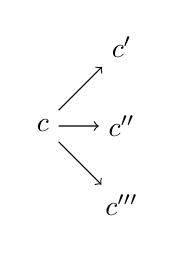
\begin{tikzpicture}[grow=right, ->, level distance=1cm,
            level 1/.style={sibling distance=1cm}]
            \node {$c$}
              child {node {$c'''$}}
              child {node {$c''$}}
              child {node {$c'$}};
        \end{tikzpicture}
    \end{center}    
\end{itemize}

\paragraph{Esempio: Reachability Problem} Dato un grafo diretto $G=(V,E)$, e due nodi $u,v\in V$, decidere se $u$ raggiunge $v$ (se esiste un cammino da $u$ a $v$). Studiamo la complessità in tempo e spazio di questo problema utilizzando sia un modello deterministico che nondeterministico.
\subparagraph{Modello deterministico} Un possibile algoritmo per risolvere questo problema è BFS$(G,u)$. Si costruisce un albero con radice $u$, e ad ogni livello si aggiungono i nodi raggiungibili in un passo. Utilizzando dei colori, alla fine della visita tutti i nodi visitati saranno neri, e quelli non raggiungibili grigi: è sufficiente controllare se $v$ è nero. Se $v$ è raggiungibile da $u$, allora $v$ sarà raggiunto da $u$ in un numero di passi $\leq |V|$. Quindi, la \textbf{complessità in tempo} è $O(|V|+|E|)$, ovvero lineare rispetto alla dimensione del grafo. Con una macchina di Turing:
\begin{center}
    \begin{tikzpicture}
        \draw (0,1) -- (7,1);
        \draw (0,1.5) -- (7,1.5);
        \foreach \x in {0.5,1} {
          \draw (\x,1) -- (\x,1.5);
        };
        \node[above] at (0.75,1) {$\rhd$};
        \node[above] at (3.75,1) {$\dots$};
        \draw [decorate,
            decoration = {brace,amplitude=5pt}] (1,1.6) -- (3.95,1.6);
        \node[above] at (2.5,1.75) {$G$};
        \draw [decorate,
            decoration = {brace,amplitude=5pt}] (4.05,1.6) -- (4.95,1.6);
        \node[above] at (4.5,1.75) {$u$};
        \draw [decorate,
            decoration = {brace,amplitude=5pt}] (5.05,1.6) -- (6,1.6);
        \node[above] at (5.5,1.75) {$v$};
        \draw [decorate,
            decoration = {brace,mirror,amplitude=5pt}] (1,.9) -- (6,.9);
        \node[below] at (3.5,.75) {$n$};

        \draw (0,-1) -- (7,-1);
        \draw (0,-.5) -- (7,-.5);
        \foreach \x in {0.5,1} {
          \draw (\x,-1) -- (\x,-.5);
        };
        \node[above] at (0.75,-1) {$\rhd$};
        \node[above] at (3.75,-1) {$\dots$};
        \draw [decorate,
            decoration = {brace,amplitude=5pt}] (1,-.4) -- (3.5,-.4);
        \node[above] at (2.25,-.25) {colori};

        \draw (0,-2.5) -- (7,-2.5);
        \draw (0,-2) -- (7,-2);
        \foreach \x in {0.5,1} {
          \draw (\x,-2.5) -- (\x,-2);
        };
        \node[above] at (0.75,-2.5) {$\rhd$};
        \node[above] at (3.75,-2.5) {$\dots$};
        \draw [decorate,
            decoration = {brace,amplitude=5pt}] (1,-1.9) -- (3,-1.9);
        \node[above] at (2,-1.75) {$Q$};
    \end{tikzpicture}
\end{center}
con $Q$ queue. Quindi, per la tesi di Church-Turing estesa, la complessità è $O(n^\alpha)$ per qualche $\alpha\in\mathbb{N}$. Si ha che
$$
    \text{Reachability} \in \text{P}
$$
Per quanto riguarda la \textbf{complessità in spazio}, si ha che i colori e $Q$ sono molto gradi, quindi
$$
    \text{Reachability} \in \text{PSPACE}
$$
\textbf{Esercizio}: migliorare questo risultato. In particolare, $\text{Reachability} \in \mathbb{L} = \text{SPACE}(\log n)$? $\text{Reachability} \in \text{SPACE}((\log n)^2)$?
\subparagraph{Modello nondeterministico} Si hanno diversi possibili stati futuri. Immaginiamo un grafo con un cammino da $u$ a $v$. Una macchina deterministica segue tutti i cammini uno ad uno, e per ognuno controlla se è quello corretto. Una macchina nondeterministica è in grado di ``indovinare'' il cammino corretto e di seguirlo.

Analizziamo la \textbf{complessità spaziale}. In questo caso non si ha bisogno dei colori. La macchina nondeterministica genera ad ogni passo un nuovo nodo nel working tape:
\begin{center}
    \begin{tikzpicture}
        \draw (0,1) -- (10.5,1);
        \draw (0,1.5) -- (10.5,1.5);
        \foreach \x in {0.5,1,2,2.5,3.5,4,5,5.5,6,7,7.5,8.5,9,10} {
          \draw (\x,1) -- (\x,1.5);
        };
        \node[above] at (0.75,1) {$\rhd$};
        \node[above] at (2.25,.9) {(};
        \node[above] at (3.75,1) {;};
        \node[above] at (5.25,.9) {)};
        \node[above] at (5.75,1) {;};
        \node[above] at (6.5,1) {$\dots$};
        \node[above] at (7.25,1) {;};
        \node[above] at (8.75,1) {;};
        \draw [decorate,
            decoration = {brace,amplitude=5pt}] (1,1.6) -- (2,1.6);
        \node[above] at (1.5,1.75) {$|V|$};
        \draw [decorate,
            decoration = {brace,amplitude=5pt}] (2.5,1.6) -- (3.5,1.6);
        \node[above] at (3,1.75) {$a$};
        \draw [decorate,
            decoration = {brace,amplitude=5pt}] (4,1.6) -- (5,1.6);
        \node[above] at (4.5,1.75) {$b$};
        \draw [decorate,
            decoration = {brace,amplitude=5pt}] (7.5,1.6) -- (8.5,1.6);
        \node[above] at (8,1.75) {$u$};
        \draw [decorate,
            decoration = {brace,amplitude=5pt}] (9,1.6) -- (10,1.6);
        \node[above] at (9.5,1.75) {$v$};
        \draw [decorate,
            decoration = {brace,mirror,amplitude=5pt}] (2,.9) -- (7,.9);
        \node[below] at (4.5,.75) {$\substack{\text{\normalsize archi}\\\text{\footnotesize worst case }O(|V|\cdot\log |V|)=n}$};
        \node[left] at (-.5,1.25) {input};

        \draw (0,-1) -- (10.5,-1);
        \draw (0,-.5) -- (10.5,-.5);
        \foreach \x in {0.5,1} {
          \draw (\x,-1) -- (\x,-.5);
        };
        \node[above] at (0.75,-1) {$\rhd$};
        \node[above] at (5,-1) {$\dots$};
        \node[ellipse,
            draw,
            minimum width=1.6cm,
            minimum height=.75cm] (A) at (1.75,-.75) { };
        \node[ellipse,
            draw,
            minimum width=1.6cm,
            minimum height=.75cm] (A) at (3.4,-.75) { };
        \node[below] at (1.75,-1.1) {$1.$};
        \node[below] at (3.4,-1.1) {$3.$};
        \node[left] at (-.3,-.75) {working t.};
    \end{tikzpicture}
\end{center}
\begin{enumerate}
    \item Genera il codice di un nodo (ad esempio, del nodo $a$)
    \item Controlla se esiste un arcp da $u$ ad $a$
    \begin{itemize}
        \item Se non esiste, ritorna ``no''
        \item Se esiste, vai avanti
    \end{itemize}
    \item Aggiungi un altro nodo (ad esempio, il nodo $b$)
    \item Controlla se esiste un arco da $a$ ad $b$
    \begin{itemize}
        \item Se non esiste, ritorna ``no''
        \item Se esiste, vai avanti
    \end{itemize}
    \item Sostituisci $a$ con $b$, e aggiungi un altro nodo (ad esempio, il nodo $c$)
    \item \dots
\end{enumerate}
\subparagraph{Esempio} Consideriamo il grafo
\begin{center}
    \begin{tikzpicture}[node distance={20mm}, main/.style = {}] 
        \node[main] (u) {$u$}; 
        \node[main] (a) [above right of=u] {$a$}; 
        \node[main] (b) [below right of=u] {$b$}; 
        \node[main] (c) [below left of=b] {$c$}; 
        \node[main] (d) [below right of=b] {$d$}; 
        \node[main] (e) [above right of=a] {$e$};
        \node[main] (f) [below right of=a] {$f$};
        \node[main] (v) [right of=f] {$v$}; 
        \draw[->] (u) -- (a);
        \draw[->] (a) -- (b);
        \draw[->] (b) -- (u);
        \draw[->] (d) -- (b);
        \draw[->] (b) -- (c);
        \draw[->] (c) -- (d);
        \draw[->] (a) -- (e);
        \draw[->] (a) -- (f);
        \draw[->] (f) -- (v);  
    \end{tikzpicture} 
\end{center}
Proviamo a trovare un cammino da $u$ a $v$:
\begin{itemize}
    \item Esiste un arco da $u$ ad $a$? Sì, quindi $ua$
    \item Esiste un arco da $a$ a $e$? Sì, quindi $uae$
    \item Esiste un arco da $e$ a $c$? No, quindi non esiste un cammino $uaec$
\end{itemize}
Esiste invece una computazione che genera il cammino $uafv$? Sì.
Si può notare come ci sia però un problema, ovvero i cicli (ad esempio $uabuabcdbcdb\dots$). In realtà, questo non è un problema: ragionando sulla complessità, e non sulla computabilità, consideriamo solo macchine di Turing che terminano.

Un modo per evitare i cicli è quello di immagazzinare in un working tape un contatore di passi eseguiti. Quando tale contatore raggiunge $|V|+1$, si può fermare la computazione e ritornare ``no''. 
$$
    \text{Reachability} \in \text{N}\mathbb{L} = \text{NSPACE}(\log n)
$$

\begin{definition}[Macchina Nondeterministica]
    Una macchina nondeterministica è una tupla $\mathcal{N}(K,\Sigma,\Delta,s)$, dove
    \begin{itemize}
        \item $K$ è un insieme finito di stati, di cui $s\in K$ è quello iniziale
        \item $\Sigma$ è un alfabeto finito, e $\rhd,\sqcup\in\Sigma$.
        \item $\Delta$ è la relazione di transizione, definita come 
        $$
        \Delta\subseteq K\times\Sigma^k\times (K\cup\{\text{yes},\text{no},\text{halt}\}) \times \Sigma^k \times \{\gets,\to,-\}^k
        $$
    \end{itemize}
    La relazione di transizione tra due configurazioni è definita come per le macchine deterministiche:
    $$
        (q,u_1,w_1,\dots,q_k,w_k) \to (q',u_1',w_1',\dots,q_k',w_k')
    $$
    con $(q',u_1',w_1',\dots,q_k',w_k')$ uno dei possibili risultati dell'applicazione di $\Delta$.
\end{definition}

\begin{definition}[Linguaggio deciso da una Macchina Nondeterministica]
    Un lin\-guag\-gio $L\subseteq(\Sigma\backslash\{\sqcup\})^*$ è deciso da una macchina nondeterministica $\mathcal{N}$ (con $\mathcal{N}(x)$ che termina sempre)
    \begin{itemize}
        \item[] se $\forall x\in L(\Sigma\backslash\{\sqcup\})^*$
        \begin{itemize}
            \item $x\in L$ $\Rightarrow$ esiste una computazione di $\mathcal{N}$ che inizia da $(s,\rhd,x,\rhd,\varepsilon,\dots,\rhd,\varepsilon)$ e termina in $(\text{yes},\dots)$
            \item $x\notin L$ $\Rightarrow$ tutte le computazioni di $\mathcal{N}$ che iniziano da $(s,\rhd,x,\rhd,\varepsilon,\dots,\rhd,\varepsilon)$ terminano in $(\text{no},\dots)$
        \end{itemize}
    \end{itemize}
\end{definition}
Se si ha una macchina che decide un linguaggio, bisogna definire la complessità spaziale e temporale su quella macchina. Per le macchine deterministiche, si ha che la complessità temporale è la lunghezza della computazione ne laso peggiore, per ogni possibile stringa di lunghezza $n$:
\begin{center}
    \begin{tikzpicture}[]
        \node (a1) at (0,0) {$\bullet$};
        \node (a2) at (0,-1) {$\bullet$};
        \node (a3) at (0,-2) {$\bullet$};
        \node (a4) at (0,-3) {$\bullet$};
        \node (b1) at (2,0) {$\bullet$};
        \node (b2) at (2,-1) {$\bullet$};
        \node (b3) at (2,-2) {$\bullet$};
        \node (b4) at (2,-3) {$\bullet$};
        \node (b5) at (2,-4) {$\bullet$};
        \node (b6) at (2,-5) {$\bullet$};
        \draw (a1) -- (a2) -- (a3) -- (a4);
        \draw (b1) -- (b2) -- (b3) -- (b4) --(b5) -- (b6);
        \node [above] at (a1) {$x\in L$};
        \node [left] at (a4) {yes};
        \node [above] at (b1) {$x\not\in L$};
        \node [right] at (b6) {no};
    \end{tikzpicture}
\end{center}
Ma nel caso nondeterministico si hanno degli alberi:
\begin{center}
    \begin{tikzpicture}[]
    \tikzstyle{level 1}=[sibling distance=4cm, level distance=1.2cm]
    \tikzstyle{level 2}=[sibling distance=1.6cm]
    \tikzstyle{level 3}=[sibling distance=1.6cm]
        \node (root) {$\bullet$}
        child {
            node (firstnode) {$\bullet$}
            child {
                node {no}        
                edge from parent 
            }
            child {
                node {$\bullet$}
                child {
                    node {$\bullet$}
                    child {
                        node {no}
                        edge from parent
                    }
                    child {
                        node {yes}
                        edge from parent
                    }
                    edge from parent
                }
                edge from parent 
            }        
            child {
                node {yes}
                edge from parent
            }
            edge from parent 
        }
        child {
            node {$\bullet$} 
            child {
                node {no}
                edge from parent
            }
            child {
                node {$\bullet$}
                child {
                    node {no}
                    edge from parent
                }
                child {
                    node {$\bullet$}
                    child {
                        node {no}
                        edge from parent
                    }
                    edge from parent
                }
                edge from parent         
            }
            edge from parent         
        }
        child {
            node {no}
            edge from parent
        };

    \node [above] at (root) {$x\in L$};
    \node [right] at (root.east) {$(s,\rhd,x,\dots)$};
    \node [left] at (firstnode) {$(q_1,w_1,\dots)$};
    \end{tikzpicture}
\end{center}

\begin{center}
    \begin{tikzpicture}[]
    \tikzstyle{level 1}=[sibling distance=4cm, level distance=1.2cm]
    \tikzstyle{level 2}=[sibling distance=1.6cm]
    \tikzstyle{level 3}=[sibling distance=1.6cm]
        \node (root) {$\bullet$}
        child {
            node (firstnode) {$\bullet$}
            child {
                node {no}        
                edge from parent 
            }
            child {
                node {$\bullet$}
                child {
                    node {$\bullet$}
                    child {
                        node {no}
                        edge from parent
                    }
                    child {
                        node {no}
                        edge from parent
                    }
                    edge from parent
                }
                edge from parent 
            }        
            child {
                node {no}
                edge from parent
            }
            edge from parent 
        }
        child {
            node {$\bullet$} 
            child {
                node {no}
                edge from parent
            }
            child {
                node {$\bullet$}
                child {
                    node {no}
                    edge from parent
                }
                child {
                    node {$\bullet$}
                    child {
                        node {no}
                        edge from parent
                    }
                    edge from parent
                }
                edge from parent         
            }
            edge from parent         
        }
        child {
            node {no}
            edge from parent
        };

    \node [above] at (root) {$x\not\in L$};
    \node [right] at (root.east) {$(s,\rhd,x,\dots)$};
    \node [left] at (firstnode) {$(q_1,w_1,\dots)$};
    \end{tikzpicture}
\end{center}
In questo caso, la complessità si può definire come l'altezza dell'albero.

\begin{definition}[Complessità Temporale di una Macchina Nondeterministica]
    U\-na\\macchina di Turing nondeterministica $\mathcal{N}$ con input $x$ richiede tempo $t$ se ogni possibile computazione di $\mathcal{N}$ su $x$ ha lunghezza al massimo $t$. 
    $\mathcal{N}$ richiede tempo $f(n)$ se, per ogni $x$, $\mathcal{N}$ termina su $x$ in tempo $f(|x|)$.
\end{definition}

\paragraph{Esempio} Immaginiamo che il grado del nondeterminismo di una macchina $\mathcal{N}$ sia 3, ovvero i nodi del suo albero hanno grado 3 ($d=3$). L'altezza è $f(|x|)$, e il numero di foglie è $d^{f(|x|)}$ (molto grande).


\begin{definition}[$\text{NTIME}(f(n))$]
    $L\in\text{NTIME}(f(n))$ se esiste una macchina di Turing nondeterministica $\mathcal{N}$ che decide $L$ in tempo $f(n)$.
\end{definition}
Notare che, ad esempio, $\text{TIME}(n^5)\neq\text{NTIME}(n^5)$. Quest'ultimo è l'insieme di tutti i linguaggi che possono essere decisi in tempo $n^5$ da una macchina di Turing nondeterministica.

\begin{proposition}
    $$
        \text{TIME}(f(n)) \subseteq \text{NTIME}(f(n))
    $$
\end{proposition}
Abbiamo che
$$
    \text{P} = \bigcup_{h\in\mathbb{N}} \text{TIME}(n^h)
    \qquad \qquad 
    \text{NP} = \bigcup_{h\in\mathbb{N}} \text{NTIME}(n^h)
$$
Quindi
$$
    \text{P} \subseteq \text{NP}
$$
Abbiamo definito la complessità temporale di una macchina nondeterministica. Possiamo definire anche la complessità spaziale come la configurazione (nodo dell'albero) massima.
\begin{definition}[Complessità Spaziale di una Macchina Nondeterministica]
    Una\\macchina di Turing nondeterministica con I/O $\mathcal{N}$ sull'input $x$ utilizza spazio $s$ se 
    $$
        s \geq \sum_{h=2}^{k-1} |w_h| + |u_h|
    $$
    Ovvero $s$ è il massimo su tutte le possibili computazioni di $\mathcal{N}$ su $x$
    $$
        s = \max\left( \sum |w_h| + |u_h| \right)
    $$
\end{definition}
$\mathcal{N}$ lavora in NSPACE$f(n)$, $\mathcal{N}$ decide $L$ in NSPACE$f(n)$.
\begin{align*}
    \text{PSPACE}=\mathbb{L} & ~\text{ spazio polinomiale su modello deterministico}\\
    \text{NPSPACE}=\text{N}\mathbb{L} & ~\text{ spazio polinomiale su modello nondeterministico} 
\end{align*}


\textcolor{Red}{TODO: finire lezione 13}


% LEZIONE 14
\textcolor{Red}{TODO: lezione 14}

% LEZIONE 15
\textcolor{Red}{TODO: lezione 15}

% LEZIONE 16
\textcolor{Red}{TODO: lezione 16}
